\section{Introduzione}
\label{sec:introduzione}

%Breve riassunto del paper
%Perché può essere utile un approccio euristico
%"In questa relazione presentiamo..."

In questa relazione verranno discusse alcune euristiche utilizzate per effettuare inferenza euristica su reti Bayesiane tramite la riduzione di Neumaser Trotter. 

In questa sezione introduttiva verrà descritto brevemente il contesto di progetto. Nella Sezione \ref{sec:euristiche}, verranno proposte e descritte diverse euristiche. Nella Sezione \ref{sec:risultati}, verranno presentati i risultati dei test svolti sulle differenti euristiche. Infine, nella Sezione \ref{sec:conclusioni} verranno tratte alcune conclusioni finali sul progetto svolto.

\subsection{La riduzione di Neumaser Trotter per effettuare inferenza su reti Bayesiane}

Una rete Bayesiana è un modello grafico probabilistico che rappresenta le dipendenze condizionali fra un gruppo di variabili. Tale rete è modellata tramite un grafo diretto ed aciclico, dove i nodi corrispondono alle variabili, e un arco fra due nodi rappresenta una dipendenza condizionale. È quindi specificata una distribuzione condizionale per ogni nodo dati i suoi genitori (i.e., altri nodi che puntano ad esso). La Figura~\ref{fig:reteB} mostra un esempio di rete Bayesiana in cui le varie distribuzioni condizionali sono rappresentate tramite delle tabelle di probabilità condizionale.

\begin{figure}[htbp]
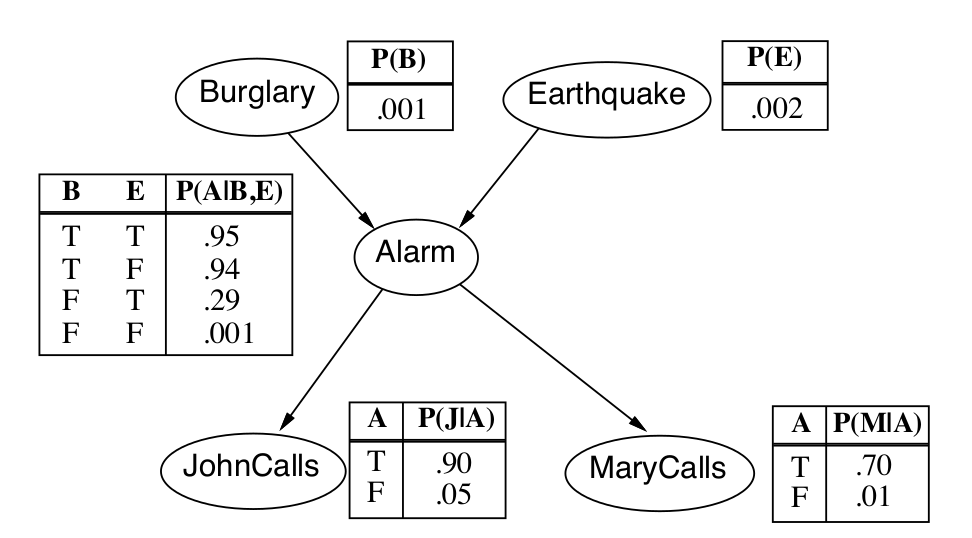
\includegraphics[width=\textwidth]{res/img/reteBayesiana.png}
\label{fig:reteB}
\caption{Esempio di rete Bayesiana.}
\end{figure}

Un problema di inferenza su reti Bayesiane è quello della Maximum A Posteriori estimate (MAP), dove, dati dei valori per alcune variabili, è necessario determinare i valori più probabili per le variabili rimanenti. È possibile considerare tale compito come un problema di ottimizzazione, in cui è necessario trovare un'assegnazione alle variabili che massimizzi un prodotto di probabilità. Inoltre, è possibile trasformare il problema di ottimizzazione in un ``Weighted CSP'', trattando i logaritmi negativi delle probabilità come costi: in questo modo, il prodotto da ottimizzare diventa una somma.

A partire da queste idee, T.K. Kumar\footnote{Kumar, TK Satish. "Kernelization, generation of bounds, and the scope of incremental computation for weighted constraint satisfaction problems." The International Symposium on Artificial Intelligence and Mathematics. 2016.} ha proposto un approccio che consiste nel convertire la rete Bayesiana in un Constraint Composite Graph (CCG), trasformare il problema in un Maximum Weigthed Vertex Cover Problem sul CCG e applicare la riduzione di Nemauser-Trotter, che determina il valore ottimo di alcune variabili.

Dopo aver applicato l'approccio proposto da Kumar, il CCG si troverà in uno stato in cui parte della variabili sono state fissate dalla riduzione di Neumaser-Trotter, mentre altre non sono ancora fissate. L'obiettivo di progetto è quello di valutare diverse euristiche per realizzare un approccio euristico: a seguito della riduzione, alcune altre variabili verranno fissate secondo una certa euristica, per poi riapplicare la riduzione di Neumaser-Trotter, e così via. 